\begin{figure}[htbp]
    \begin{center}
        \subfigure[Resultados de aptitud para el experimento]{%
            \label{fig:exp10_zero}
            \scalebox{2}{\begin{tikzpicture}
\node at (0,0) {\includegraphics[width=4.1cm, trim={0 0 0 0}, clip]{Hamming_min2.PNG}};
\node at (4,0) {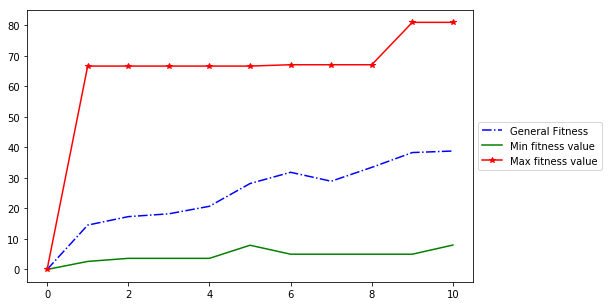
\includegraphics[width=4.1cm, trim={0 0 0 0}, clip]{Fitness.PNG}};
%\node[rotate=30] at (1,2) {\includegraphics[width=3cm]{example-image}};
\end{tikzpicture}}
            %\scalebox{2.0}{\begin{tikzpicture}
\node at (0,2) {
\includegraphics[width=3cm, trim={0 0 0 60}, clip]{Gen1Ind1_BF.PNG}};
\node at (0,0) {
\includegraphics[width=3cm, trim={0 0 0 60}, clip]{Gen1Ind1_AF.PNG}};
%\node[rotate=30] at (1,2) {\includegraphics[width=3cm]{example-image}};
\end{tikzpicture}}
        }\\%
        %\subfigure[Resultados de aptitud para el experimento]{%
        %    \label{fig:exp10_first}
            %\scalebox{0.8}{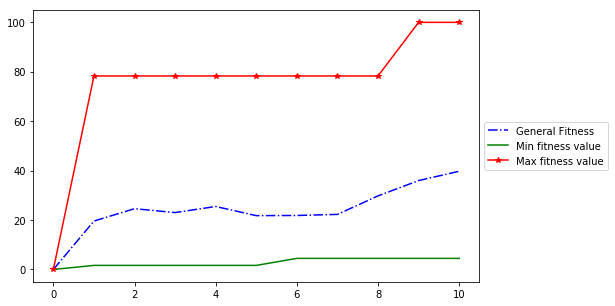
\includegraphics[width=0.8\textwidth]{Fitness.png}}
        %    \includegraphics[width=0.5\textwidth]{Hamming_min.png}
        %}\\%
        %\subfigure[Distancia Hamming promedio en el experimento]{%
        %\label{fig:second}
        %\scalebox{0.8}{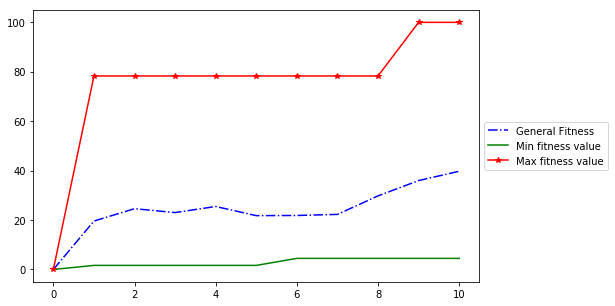
\includegraphics[width=0.8\textwidth]{Fitness.png}}
        %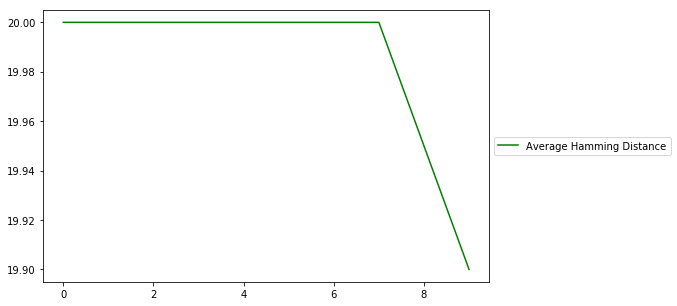
\includegraphics[width=0.6\textwidth]{Hamming.png}
        %}\\ 
            
        %  ------- End of the first row ----------------------%
        \subfigure[Individuos de la generación 1]{%
            \label{fig:exp10_third}
            \scalebox{1.8}{\begin{tikzpicture}
\node at (0,2) {
\includegraphics[width=3cm, trim={0 0 0 60}, clip]{Gen1Ind1_BF.PNG}};
\node at (0,0) {
\includegraphics[width=3cm, trim={0 0 0 60}, clip]{Gen1Ind1_AF.PNG}};
%\node[rotate=30] at (1,2) {\includegraphics[width=3cm]{example-image}};
\end{tikzpicture}}
            %\scalebox{2.0}{\begin{tikzpicture}
\node at (0,2) {
\includegraphics[width=3cm, trim={0 0 0 60}, clip]{Gen1Ind1_BF.PNG}};
\node at (0,0) {
\includegraphics[width=3cm, trim={0 0 0 60}, clip]{Gen1Ind1_AF.PNG}};
%\node[rotate=30] at (1,2) {\includegraphics[width=3cm]{example-image}};
\end{tikzpicture}}
        }%
        \subfigure[Individuos generación 10 (no repetidos)]{%
            \label{fig:exp10_fourth}
            \scalebox{1.8}{\begin{tikzpicture}
\node at (0,3) {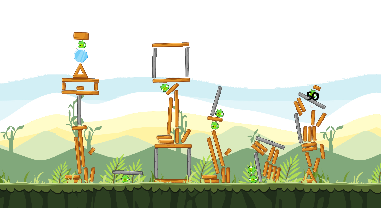
\includegraphics[width=3cm, trim={0 0 5 10}, clip]{Gen1Worst_Before.PNG}};
\node at (0,0) {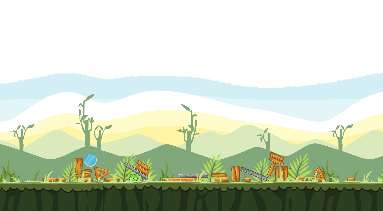
\includegraphics[width=3cm, trim={0 0 0 60}, clip]{Gen1Worst_After.PNG}};
%\node[rotate=30] at (1,2) {\includegraphics[width=3cm]{example-image}};
\end{tikzpicture}}
        }
    \end{center}
    \caption{Evolución de los individuos de un experimento }
    \label{figure:exp_10_a}
\end{figure}
